%15) Que tipos de linguagens existem no contexto de Sistemas de Bancos de Dados (DDL, DML, etc.)? Quais os objetivos de cada linguagem?
%16) O que é um Modelo de Dados? Defina o objetivo de um Modelo de Dados.
%17) Explique o que é a atividade de Projeto de Banco de Dados. Caracterize os níveis de abstração envolvidos: descritivo, conceitual, operacional e físico.
%18) Descreva os principais componentes de um SGBD, explicitando sua funcionalidade. Desenhe um diagrama ilustrando as relações entre os componentes do SGBD.
%19) Explique a arquitetura ANSI/SPARC.
%20) O que é independência de dados? Dê exemplo de independência de dados física e lógica no contexto da arquitetura ANSI/SPARC de SGBD

\documentclass[12pt]{article}
\usepackage[brazil]{babel}
\usepackage[a4paper, total={6in, 8in}]{geometry}
\usepackage[utf8]{inputenc}

\usepackage{graphicx}
\usepackage{url}
\usepackage{float}
\usepackage{listings}
\usepackage{color}
\usepackage{algorithmic}
\usepackage{algorithm}
\usepackage{hyperref}
\usepackage{graphicx}

\begin{document}

\title{Tarefas do Módulo 3 BD}
\author{Pedro Henrique de Brito Agnes}

\maketitle

\setcounter{section}{14}
\section{Tipos de Linguagens SBD}
Os tipos de linguagem de um SBD são:
\begin{itemize}

\item
\textbf{DDL}, \textit{Data Definition Language} - Tem como objetivo, definir a estrutura dos dados e esquemas do BD.

Dentre os comandos DDL, temos \texttt{CREATE}, \texttt{ALTER} e \texttt{DROP}

\item
\textbf{DML}, \textit{Data Manipulation Language} - Tem como objetivo, acessar e manipular os dados das tabelas.

São comandos DML : \texttt{SELECT}, \texttt{INSERT}, \texttt{DELETE} e \texttt{UPDATE}

\item
\textbf{DTL}, \textit{Data Transaction Language} - Tem como objetivo, o controle de transação, que roda as mudanças feitas pelo DML.

São comandos DTL : \texttt{BEGIN TRANSACTION}, \texttt{COMMIT} e \texttt{ROLLBACK}

\item
\textbf{DCL}, \textit{Data Control Language} - Tem como objetivo, controlar a parte de segurança do banco de dados, retornando os dados salvos ou guardados.

São comandos DCL : \texttt{GRANT}, \texttt{REVOKE} e \texttt{DENY}

\item 
\textbf{SDL}, \textit{Storage Definition Language} - Tem como objetivo, especificar o esquema interno.

\item
\textbf{VDL}, \textit{View Definition Language} - Tem como objetivo, especificar a visão do usuário e seu mapeamento para um esquema conceitual.

\end{itemize}

\section{Modelo de Dados}
Um modelo de dados é o modelo para organização dos dados de um BD que pode ter diferentes tipos de abstração. É classificado como alto nível, nível médio e baixo nível.

O alto nível representa a forma como os dados são compreendidos pelos usuários. Já o nível médio é implementado pelo SGBD e é divido em vários tipos, como modelo relacional, hierárquico, orientado a objetos, entre outros. Por fim, o baixo nível, simplesmente descreve como os dados são armazenados fisicamente.

O principal objetivo de um modelo de dados é o de disponibilizar uma representação conceitual dos dados.

\section{Atividade de Projeto de BD}
A atividade de projeto de banco de dados é usada para o desenvolvimento do mesmo, onde se é projetada toda a sua estrutura. Para isso, são executadas certas tarefas, como a construção do esquema, definição de como serão armazenados os dados e direitos de acessos.
Para facilitar esta atividade, são usados diferentes níveis de abstração: descritivo, conceitual, operacional e físico.

No modelo descritivo, é usada uma linguagem mais natural, com objetos do mudo real para possibilitar um melhor entendimento para leigos. De forma geral, informações informais.

No modelo conceitual é usada uma linguagem mais formal, explicitando a organização e algumas estruturas armazenadas no banco de dados.

No modelo operacional, são mostradas as especificações de manipulação para o computador. 

Por fim, no modelo físico, é mostrado como os dados estão de fato, armazenados. Mostra-se as estruturas internas, tabelas, entre outros.

\section{Componentes de um SGBD}
Os principais componentes de um SGBD são:
\begin{itemize}
\item \textbf{Pré-compilador} - É o compilador da linguagem de programação utilizada, que tem como funcionalidade, realizar as operações juntamente com o compilador DML.
\item \textbf{Compilador DDL} - Responsável por processar e armazenar as definições do esquema especificado.
\item \textbf{Processamento de banco de dados em tempo de execução} - Controla os acessos ao banco e executa os comandos recebidos no BD.
\item \textbf{Gerenciador de dados armazenados} - Utilizando serviços do sistema ope-racional, controla a transferência de dados entre o disco e a memória principal.
\item \textbf{Controle de Concorrência/\textit{Backup}/Subsistema de Recuperação} - É responável pelos backups de dados do banco quando necessário.
\end{itemize}

\begin{figure}[H]
    \centering
    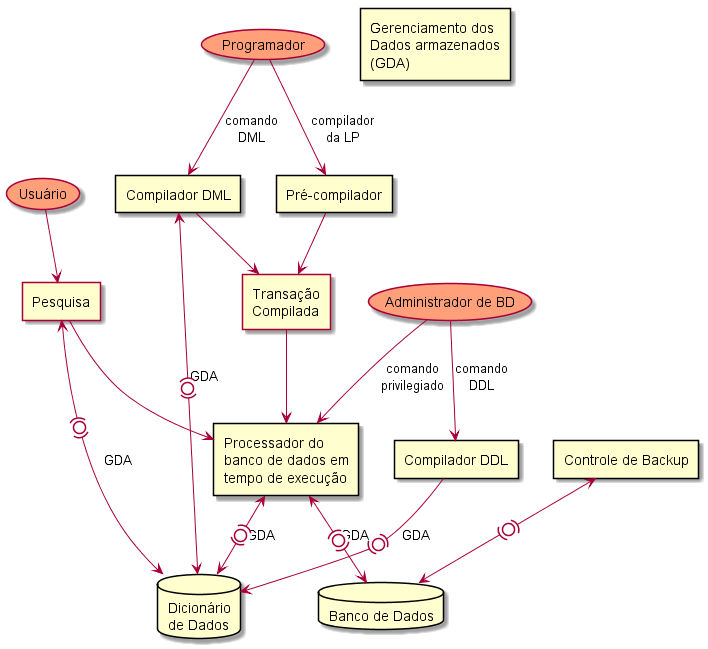
\includegraphics[width=.7\textwidth]{Diagrama18/diagrama18.png}
    \caption{Diagrama das relações entre os componentes do SGBD.}
\end{figure}

\section{Arquitetura ANSI/SPARC}
A arquitetura ANSI/SPARC é responsável pela divisão das aplicações de usuário em níveis, sendo interno, conceitual e externo que, de forma resumida, permite diferentes visões do banco de dados dependendo do interesse de cada grupo. Assim, é mostrada a parte do banco de interesse e é escondida o que menos interessa.

De forma resumida, o nível externo descreve a visão dos usuários da aplicação do BD, o conceitual, a visão dos desenvolvedores e o interno, da máquina.

\section{Independência de dados}
A independência de dados é caracterizada pela possibilidade de alterar um esquema em um nível inferior sem alterar um nível superior.

Existem dois tipos de independência de dados no contexto da arquitetura ANSI/SPARC, física e lógica. Na independência de dados física, é possível alterar o esquema interno sem ter que alterar o conceitual. Já na independência de dados lógica, é possível alterar o esquema conceitual sem alterar o externo.

\end{document}